\chapter{cyclic evolution}\label{CE}
本章では,cyclic evolutionを説明する.特に,LZ遷移を含むcyclic evolutionは,その代表例である.


\section{序論}
本論文では,cyclic evolutionとは,時間発展の後,Hamiltonianが初期状態に戻るような系のことを指すものとする\footnote{多くの場合,cyclic evolutionは,状態ベクトルが初期状態に戻るような時間発展を指す.}.このようなHamiltonianは,Pauli行列を基底としたパラメータ空間内で閉曲線を描く.


第\ref{AT}章で,Berry位相を定義した.この位相を,断熱条件が成り立たない場合に拡張したものをAharonov-Anandan位相と呼ぶ.系の状態ベクトルが初期状態に戻るような系でAharonov-Anandan位相が定義できる\cite{Aharonov}.



\section{LZ遷移を含むcyclic evolution}
cyclic evolutionの例として,LZ遷移を周期的に繰り返す系を考えよう\cite{Kayanuma1993}.この系のHamiltonianは,
\begin{align}
  \Hat{H}_{\mathrm{CE}}
  &=
  \begin{pmatrix}
    \varepsilon_0 \cos \omega t& \Delta_0 C(t)\\
    \Delta_0 C(t) & -\varepsilon_0 \cos \omega t
  \end{pmatrix} \\
  &= \Delta_0 C(t) \, \Hat{\sigma}_x + \varepsilon_0 \cos \omega t \, \Hat{\sigma}_z \label{H_CE_LZ}
\end{align}
で表される.ただし,$\omega$は角振動数である.


この系における断熱エネルギーの時間変化は図\ref{fig:CE_LZ}のようになる.図\ref{fig:CE_LZ}から,断熱エネルギーは周期的に準位交差することがわかる.また,パウリ行列を基底とするパラメータ空間にHamiltonianを描写すると図\ref{fig:CE_LZ_Pauli}のようになる.図\ref{fig:CE_LZ_Pauli}より,Hamiltonianが閉曲線を描いているため,この系はcyclic evolutionである.

\begin{figure}[htbp]
  \centering
  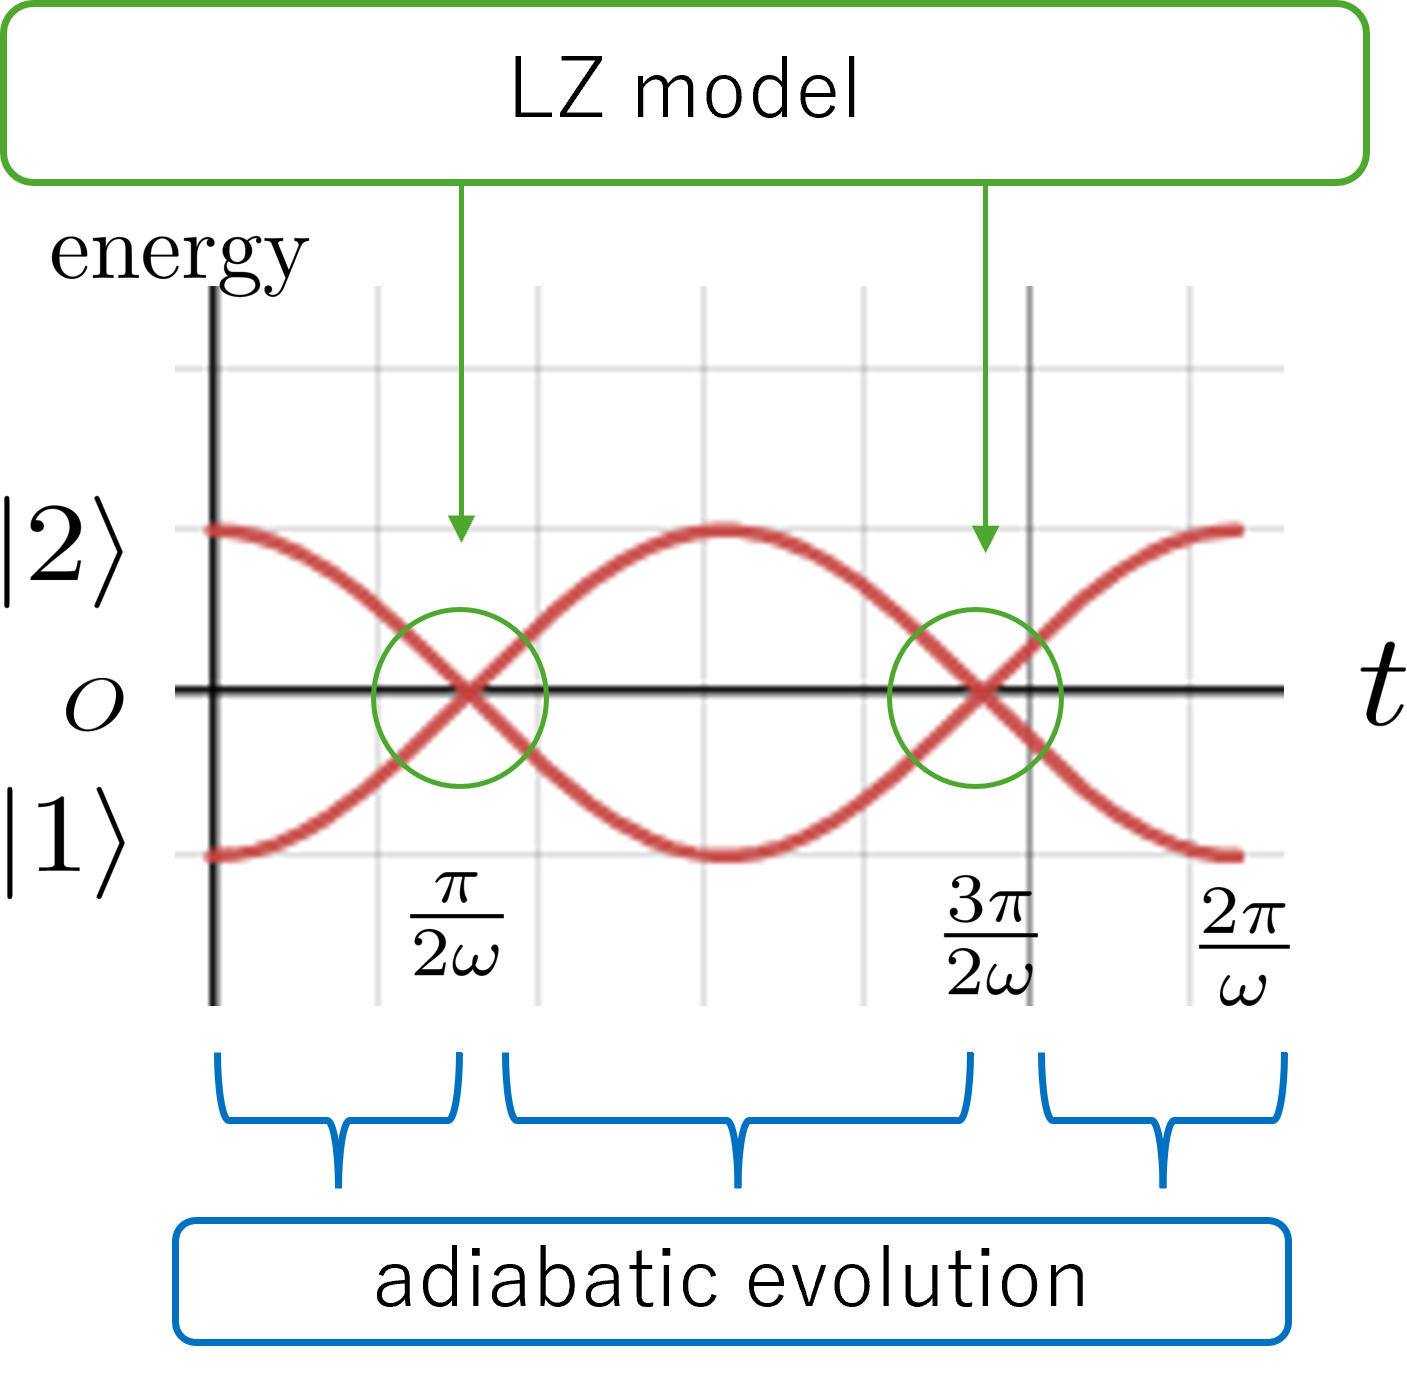
\includegraphics[scale=0.7]{figures/CE_LZ.png}
  \caption{LZ遷移を含むcyclic evolutionにおける断熱エネルギーの時間変化}
  \label{fig:CE_LZ}
\end{figure}

\begin{figure}[htbp]
  \centering
  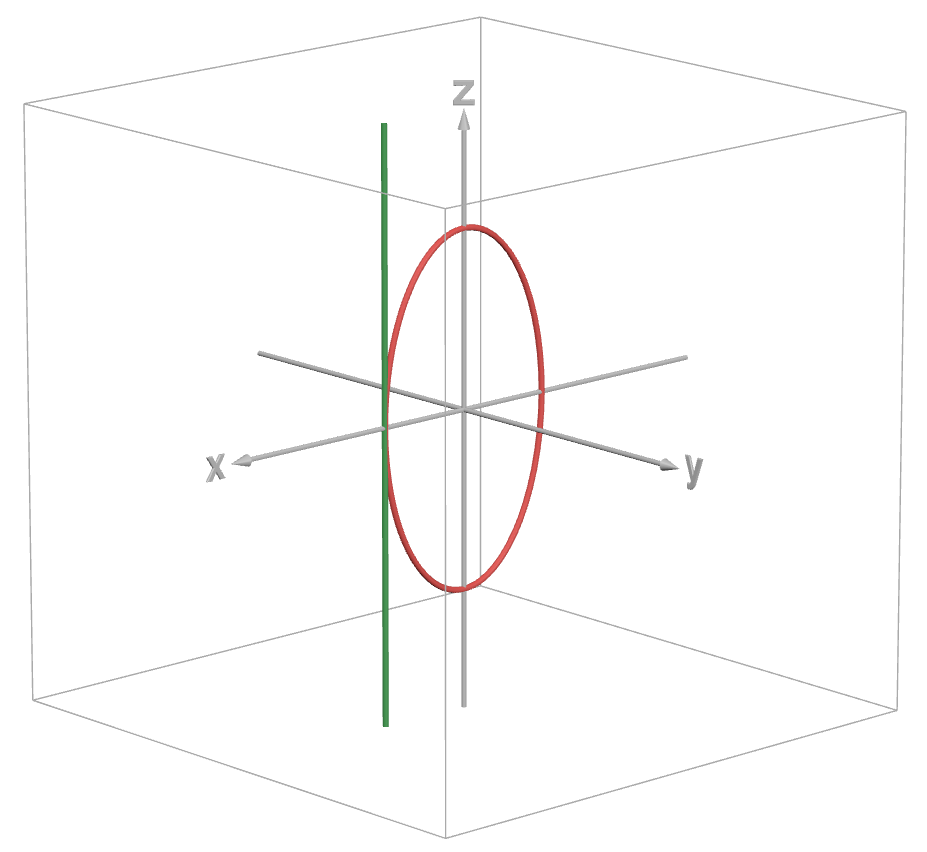
\includegraphics[scale=0.3]{figures/CE_LZ_Pauli.png}
  \caption{LZ遷移を含むcyclic evolutionにおけるHamiltonanの経路を赤い線で示している.緑の線は1回のLZ遷移である.}
  \label{fig:CE_LZ_Pauli}
\end{figure}


この系における,各準位交差後の波動関数を求めよう.ここで,$\Delta_0 \ll \varepsilon_0 $のとき,転送行列法を用いることができる.転送行列法では,この系を3つの部分
\begin{enumerate}
  \item 断熱エネルギー差がもっとも大きくなる時点から準位交差直前までの断熱的な時間発展
  \item 準位交差付近のLZ遷移
  \item 準位交差直後から,断熱エネルギー差がもっとも大きくなる時点までの断熱的な時間発展
\end{enumerate}
に分割する.また,$2 \times 2$行列
\begin{align}
  M &= 
  \begin{pmatrix}
    \sqrt{q} & -\sqrt{1-q} e^{i\phi_s}\\
    \sqrt{1-q} e^{i\phi_s} & \sqrt{q}
  \end{pmatrix},\\
  H &=
  \begin{pmatrix}
    e^{i\eta}  & 0\\
    0 & e^{-i\eta}
  \end{pmatrix},\\
  G &= 
  \begin{pmatrix}
    e^{i\theta}  & 0\\
    0 & e^{-i\theta}
  \end{pmatrix}
\end{align}
を定義する.ただし,
\begin{align}
  q &:= \exp(-2\pi \bar{\delta}),\\
  \bar{\delta} &:= \frac{\Delta_0^2}{2\varepsilon_0 \omega},\\
  \eta (t) &:= \int_0^t dt^{\prime} \sqrt{(\varepsilon_0 \cos\omega t)^2+ (\Delta_0 C(t))^2},\\
  \theta &:= 2 \int_0^{\frac{\pi}{2\omega}} dt \sqrt{(\varepsilon_0 \cos\omega t)^2+ (\Delta_0 C(t))^2} = 2 \eta(\frac{\pi}{2\omega}),\\
  \phi_s &:= \frac{\pi}{4} + \arg \Gamma(1-i\bar{\delta}) + \bar{\delta}(\ln \bar{\delta} -1)
\end{align}
である\footnote{特に,$\phi_s$は,Stokes位相と呼ばれ,Landau-Zener遷移前後における位相の変化を議論する際に重要である.}.さらに,ある行列$A$と一対一に対応する行列を$A^{\prime}$で表す\footnote{$C(t)$の具体形によって,対応する行列が変わるため,曖昧に記述している.$A^{\prime}$は,$A$の複素共役行列や転置行列である場合が多い.}.例えば,$C(t) = 1$,$C(t) = \sin \omega t$のとき,$A^{\prime}$はそれぞれ$A$の転置行列,複素共役行列になる.このとき,$t=0$における波動関数を$\psi_0 = (1,0)^T$とすると,$t = \frac{\pi}{\omega}, \frac{2\pi}{\omega}, \ldots, \frac{(2m-1)\pi}{\omega}, \frac{2m \pi}{\omega} , \ldots$における波動関数$\psi_1, \psi_2, \ldots,\psi_{2m-1} , \psi_{2m}, \ldots$は,
\begin{align}
  \psi_1 &= G^{\frac{1}{2}} M G^{\prime \frac{1}{2}} \psi_0,\\
  \psi_2 &=  G^{\prime \frac{1}{2}} M^* G M G^{\prime \frac{1}{2}} \psi(0),\\
  \vdots \notag \\
  \psi_{(2m-1)} &= (G^{\frac{1}{2}} M G^{\prime \frac{1}{2}}) (G^{\prime \frac{1}{2}} M^{\prime} G M G^{\prime \frac{1}{2}})^{m-1} \psi_0,\\
  \psi_{2m} &= (G^{\prime \frac{1}{2}} M^{\prime} G M G^{\prime \frac{1}{2}})^{m} \psi_0,\\
  \vdots \notag
\end{align}
で表される.

\section{転送行列$M$の決定}
本節では,転送行列$M$が,
\begin{equation}
  M =
  \begin{pmatrix}
    e^{-\pi\bar{\delta}} & -\sqrt{1-e^{-2\pi\bar{\delta}}} e^{i\phi_s}\\
    \sqrt{1-e^{-2\pi\bar{\delta}}} e^{-i\phi_s} & e^{-\pi\bar{\delta}} 
  \end{pmatrix}
\end{equation}
となることを示す\footnote{付録Aも参照せよ.}.


そのために,準位交差直前の状態$(c_1^-, c_2^-)$から準位交差後の状態$(c_1^-, c_2^-)$が導かれることを仮定する.すなわち,ある行列$M$を用いて,
\begin{equation}
  \begin{pmatrix}
    c_1^+\\
    c_2^+
  \end{pmatrix}
  =
  \begin{pmatrix}
    M_{11} & M_{12}\\
    M_{21} & M_{22}
  \end{pmatrix}
  \begin{pmatrix}
    c_1^-\\
    c_2^-
  \end{pmatrix}
\end{equation}
と書けるものとする.また,議論の見通しを良くするため,$\varepsilon_0 \rightarrow -v/2$とする.

まず,$M_{11}$を求める.Shr\"{o}dinger方程式(\ref{SE})に,系のHamiltonian(\ref{H_CE_LZ})を代入して,
\begin{equation}
  i\frac{d}{dt} c_1(t) = -\frac{vt}{2} c_1(t) + \Delta_0 c_2(t)
\end{equation}
となる.ここで,
\begin{align}
  z &= i\sqrt{v} e^{i\frac{\pi}{4}} t\\
  n &= i\bar{\delta}\\
  \bar{\delta} &= \frac{\Delta_0^2}{v} \label{delta_bar}\\
  c_1 &= w_1(z)\\
  c_2 &= w_2(z)
\end{align}
という変数変換を行って整理すると,
\begin{equation}
  \left( \frac{d}{dz} + \frac{z}{2} \right) w_1 = - e^{-\frac{i\pi}{4}} \frac{\Delta_0}{\sqrt{v}} w_2 \label{M11}
\end{equation}
となる.ここで,定理
\begin{equation}
  \left( \frac{d}{dz} + \frac{z}{2} \right) D_n(z) = n D_{n-1} (z)
\end{equation}
を用いると,
\begin{align}
  \text{(\ref{M11})の左辺} &= A \left( \frac{d}{dz} + \frac{z}{2}\right) D_n(z) = A n D_{n-1}(z)\\
  \text{(\ref{M11})の右辺} &= - e^{-\frac{i\pi}{4}} \frac{\Delta_0}{\sqrt{v}} B D_{n-1}(z)
\end{align}
である.したがって,
\begin{align}
  Ai\bar{\delta} &= - e^{-\frac{i\pi}{4}} \sqrt{\bar{\delta}} B\\
  \therefore B &= \sqrt{\bar{\delta}} (-i) e^{\frac{i\pi}{4}} A\\
  &= \sqrt{\bar{\delta}} e^{-\frac{i\pi}{4}} A
\end{align}
である.よって,$t \rightarrow -\infty$における$c_2(t)$は,
\begin{align}
  \lim_{t \rightarrow -\infty} c_2(t) 
  &= B \frac{\sqrt{2 \pi}}{\Gamma(1-i \bar{\delta})} \exp \left(-\frac{\pi \bar{\delta}}{4}-\frac{i v t^2}{4}-i \bar{\delta} \log \sqrt{v} t\right)\\
  &= A \frac{\sqrt{2 \pi \bar{\delta}}}{\Gamma(1-i \bar{\delta})} \exp \left(-\frac{\pi \bar{\delta}}{4} - \frac{i\pi}{4} - \frac{i v t^2}{4} - i \bar{\delta} \log \sqrt{v} t\right) \label{C2_inf}
\end{align}
である.


ここで,系(\ref{H_CE_LZ})における断熱エネルギーは
\begin{equation}
  E_{\pm}(t) = \pm \sqrt{\Delta_0^2 + \frac{v^2 t^2}{4}}
\end{equation}
で与えられる.断熱エネルギー$E_{\pm}(t)$を用いて,
\begin{align}
  F(t)
  &:= \int E_{\pm} (t) dt\\
  &= \int \sqrt{\Delta_0^2 + \frac{v^2 t^2}{4}} dt\\
  &= \frac{t}{4} \sqrt{4\Delta_0^2 + v^2 t^2} + \frac{\Delta_0^2}{v} \log |v^2 t + v \sqrt{4\Delta_0^2 + v^2 t^2}|
\end{align}
を定義する.このとき,
\begin{align}
  \chi
  &:= \int_0^t \sqrt{\Delta_0^2 + \frac{v^2 t^2}{4}} dt^{\prime}\\
  &= F(t) -F(0)\\
  &= \frac{t}{4} \sqrt{4\Delta_0^2 + v^2 t^2} + \frac{\Delta_0^2}{v} \log |v^2 t + v \sqrt{4\Delta_0^2 + v^2 t^2}| - \frac{\Delta_0^2}{v} \log(2\Delta_0 v)\\
  &= \frac{t}{4} \sqrt{4\Delta_0^2 + v^2 t^2} + \frac{\Delta_0^2}{v} \log \left(\frac{vt}{2\Delta_0} + \sqrt{\left(1 + \frac{v^2 t^2}{4\Delta_0^2}\right)}\right)\\
  &= \frac{t}{4} \sqrt{4\Delta_0^2 + v^2 t^2} + \frac{\Delta_0^2}{v} \log \left( \frac{\sqrt{v}}{\Delta_0} \left( \frac{\sqrt{v} t}{2} + \sqrt{\frac{\Delta_0^2}{v} + \frac{v t^2}{4}}\right)\right)\\
  &= \frac{t}{4} \sqrt{4\Delta_0^2 + v^2 t^2} + \frac{\Delta_0^2}{v} \left( \log  \left(\frac{\sqrt{v} t}{2} + \sqrt{\frac{\Delta_0^2}{v} + \frac{v t^2}{4}}\right) - \log \left(\frac{\Delta_0}{\sqrt{v}}\right) \right)
\end{align}
となる.ここで,
\begin{equation}
  X = \frac{\sqrt{v} t}{2}
\end{equation}
および式(\ref{delta_bar})を用いて変数変換を行うと,
\begin{equation}
  \chi = X \sqrt{X^2 + \bar{\delta}} + \bar{\delta} (\log |X + \sqrt{X^2 + \bar{\delta}}| - \log \sqrt{\bar{\delta}})
\end{equation}
となる.$X \gg \bar{\delta}$のとき,
\begin{align}
  \chi
  &\approx X^2 (1+ \frac{\bar{\delta}}{2 X^2}) + \bar{\delta} (\log \left|X + X\sqrt{1 + \frac{\bar{\delta}}{2X^2}}\right| - \bar{\delta} \log \sqrt{\bar{\delta}})\\
  &\approx X^2 + \frac{\bar{\delta}}{2} + \bar{\delta} \log |2X| - \bar{\delta} \log \sqrt{\bar{\delta}}
\end{align}
である.$t \rightarrow \infty$のとき,
\begin{equation}
  \chi =  \frac{v t^2}{4} + \frac{\bar{\delta}}{2} (1-\log \bar{\delta}) + \bar{\delta} \log(\sqrt{v}t)
\end{equation}
また,$t \rightarrow -\infty$のときの$\chi$は,符号を反転させればよい.したがって,
\begin{align}
  \lim _{t \rightarrow-\infty}\left(
  \begin{array}{l}
    c_1(t) \\
    c_2(t)
  \end{array}
  \right) &=\left(
  \begin{array}{ll}
    c_1^{-} & e^{i \chi} \\
    c_2^{-} & e^{-i \chi}
  \end{array}
  \right) \\
  \lim _{t \rightarrow \infty}\left(
  \begin{array}{l}
    c_1(t) \\
    c_2(t)
  \end{array}
  \right) &= \left(
  \begin{array}{ll}
    c_1^{+} & e^{i \chi} \\
    c_2^{+} & e^{-i \chi}
  \end{array}
  \right) \label{C1_C2}
\end{align}
を仮定すると,Landau-Zener公式より,
\begin{equation}
  \frac{\lim_{t \rightarrow \infty} c_1(t)}{\lim_{t \rightarrow -\infty} c_1(t)} = \exp (-\pi \bar{\delta})
  = \frac{c_1^+ e^{i\chi}}{c_1^- e^{i\chi}}
\end{equation}
であるから,
\begin{align}
  c_1^+ = e^{-\pi \bar{\delta}} c_1^-
\end{align}
より,
\begin{equation}
  M_{11} = e^{-i\bar{\delta}}
\end{equation}
と決定された.


次に,$M_{12}$を求めよう.
式(\ref{C2_inf})および式(\ref{C1_C2})より,
\begin{align}
  c_2^+
  &= e^{i\chi} \lim_{t \rightarrow \infty} c_2\\
  &= A \frac{\sqrt{2 \pi \bar{\delta}}}{\Gamma(1-i \bar{\delta})} \exp \left(-\frac{\pi \bar{\delta}}{4} - \frac{i\pi}{4} - \frac{i v t^2}{4} - i \bar{\delta} \log \sqrt{v} t + \frac{ivt^2}{4} + \frac{i\bar{\delta}}{2} (1 - \log \bar{\delta})  + i\bar{\delta} \log (\sqrt{v}t) \right)\\
  &= A \frac{\sqrt{2 \pi \bar{\delta}}}{\Gamma(1-i \bar{\delta})} \exp \left(-\frac{\pi \bar{\delta}}{4} - \frac{i\pi}{4} +\frac{i\bar{\delta}}{2} (1 - \log \bar{\delta}) \right)
\end{align}
である.また,式(\ref{C1_inf})および式(\ref{C1_C2})より,
\begin{align}
  c_1^-
  &= e^{-i\chi} \lim_{t \rightarrow \infty} c_1\\
  &= A \exp \left(\frac{i v t^2}{4} + \frac{\pi \bar{\delta}}{4} + i \bar{\delta} \log \sqrt{v} t - \left( \frac{i v t^2}{4} + \frac{i\bar{\delta}}{2} (1 - \log \bar{\delta})  + i\bar{\delta} \log (\sqrt{v}t) \right) \right)\\
  &= A \exp \left( \frac{\pi \bar{\delta}}{4} - \frac{i\bar{\delta}}{2} (1 - \log \bar{\delta}) \right)
\end{align}
である.したがって,$A$を消去すると,
\begin{align} 
  c_2^{+}
  &= \frac{\sqrt{2 \pi \bar{\delta}}}{\Gamma(1-i \bar{\delta})} e^{-\frac{\pi \bar{\delta}}{2}} \exp \left(-i(\bar{\delta} (\log \bar{\delta}-1))+\frac{\pi}{4}\right) c_1^{-} \\
  &= \frac{\sqrt{2 \pi \bar{\delta}}}{|\Gamma(1-i \bar{\delta})|} \frac{e^{-\frac{\pi \bar{\delta}}{2}}}{e^{i \phi_s}} c_1^{-} \\ & =\frac{\sqrt{2 \pi \bar{\delta}} e^{-\frac{\pi \bar{\delta}}{2}} e^{-i \phi_s}}{|-i \bar{\delta} \Gamma(-i \bar{\delta})|} c_1^{-} \\
  &= \frac{\sqrt{2 \pi \bar{\delta}} e^{-\frac{\pi \bar{\delta}}{2}} e^{-i \phi_s}}{\bar{\delta}} \frac{1}{|\Gamma(-i \bar{\delta}|)} c_1^{-} \\
  &= \frac{\sqrt{2 \pi \bar{\delta}} e^{-\frac{\pi \bar{\delta}}{2}} e^{-i \phi_s}}{\bar{\delta}} \sqrt{\frac{\bar{\delta} \sinh (\bar{\delta} \pi)}{\pi}} c_1^{-} \\
  &= \sqrt{2} e^{-\frac{\pi \bar{\delta}}{2}}\left(\frac{1}{2}\left(e^{\pi \bar{\delta}}-e^{-\pi \bar{\delta}}\right)\right)^{\frac{1}{2}} e^{-i \phi_s} c_1^{-} \\
  &= (e^{-\pi \bar{\delta}}\left(e^{\pi \bar{\delta}}-e^{-\pi \bar{\delta}}\right))^{\frac{1}{2}} e^{-i \phi_s} c_1^{-} \\ 
  &= \sqrt{1-e^{-2 \pi \bar{\delta}}} e^{-i \phi_s} c_1^{-}
\end{align}
より,
\begin{equation}
  c_2^+ = \sqrt{1 - e^{-2\pi \bar{\delta}}} e^{-i\phi_s} c_1^-
\end{equation}
であるから,
\begin{equation}
  M_{21} = \sqrt{1 - e^{-2\pi \bar{\delta}}} e^{-i\phi_s}
\end{equation}
と決定される.ただし,ガンマ関数の性質を用いている.


また,時間反転対称性より,$M_{22} = M_{11}$,転送行列$M$のユニタリー性から$M_{21} = -M_{12}$がそれぞれいえる.


したがって,転送行列$M$が決定された.

\subsection{$C(t) =1$の場合}
LZ遷移を含むcyclic evolutionのもっとも簡単な例は,$C(t) =1$である\cite{Kayanuma1994}.このとき,Hamiltonianは,
\begin{equation}
  \Hat{H} =
  \begin{pmatrix}
    \varepsilon_0 \cos \omega t & \Delta_0\\
    \Delta_0 & -\varepsilon_0 \cos \omega t
  \end{pmatrix} 
\end{equation}
である.また,$M$および$G$に対応する行列は,それぞれの転置行列である.そのため,初期状態を$\psi_0 = (1,0)$とすると,
\begin{align}
  \psi_1 &= G^{\frac{1}{2}} M G^{T \frac{1}{2}} \psi_0,\\
  \psi_2 &=  G^{T \frac{1}{2}} M^T G M G^{T \frac{1}{2}} \psi(0),\\
  \vdots\\
  \psi_{2m-1} &= (G^{\frac{1}{2}} M G^{T \frac{1}{2}}) (G^{T \frac{1}{2}} M^T G M G^{T \frac{1}{2}})^{m-1} \psi_0,\\
  \psi_{2m} &= (G^{T \frac{1}{2}} M^T G M G^{T \frac{1}{2}})^{m} \psi_0,\\
  \vdots
\end{align}
で表される.


この系が,$t = \frac{(2m-1)\pi}{\omega}, \frac{2m \pi}{\omega}$においてそれぞれ状態$|1\rangle$にある確率$P_{2m-1}, P_{2m}$は,
\begin{align}
  P_{2m-1} &= 1 - q \left( \frac{\cos(2m-1) \theta}{\cos\theta} \right)^2\\
  P_{2m} &= q \left( \frac{\sin 2m \theta}{\cos\theta} \right)^2
\end{align}
であることが知られている\cite{Kayanuma1994}.

\subsection{$C(t) = \sin \omega t$の場合} \label{C_sin}
$C(t) =\sin \omega t$のとき,Hamiltonianは,
\begin{equation}
  \Hat{H} =
  \begin{pmatrix}
    \varepsilon_0 \cos \omega t & \Delta_0 \sin \omega t\\
    \Delta_0 \sin \omega t & -\varepsilon_0 \cos \omega t
  \end{pmatrix}
  \label{H_1997}
\end{equation}
である\cite{Kayanuma1997}.また,$M$および$G$に対応する行列は,それぞれの複素共役行列である.そのため,初期状態を$\psi_0 = (1,0)$とすると,
\begin{align}
  \psi_1 = G^{\frac{1}{2}} M_1 G^{*\frac{1}{2}} \psi_0\\
  \psi_2 = G^{*\frac{1}{2}} M_2 G^{\frac{1}{2}} \psi_0
\end{align}
である.ここで,表式を簡単にするため,
\begin{align}
  T &= G^{\frac{1}{2}} M G^{*\frac{1}{2}}\\
  T^* &= G^{*\frac{1}{2}} M^* G^{\frac{1}{2}}
\end{align}
としよう.このとき,
\begin{align}
  \psi_{2m-1} &= T (T^* T)^{m-1} \psi_0 \label{psi_2m-1}\\
  \psi_{2m} &= (T^* T)^{m} \psi_0 \label{psi_2m}
\end{align}
と書ける.また,
\begin{align}
  S = 
  \begin{pmatrix}
    \sqrt{1-q} e^{-i(\phi_s + \theta)} & \sqrt{q}\\
    -\sqrt{q} & \sqrt{1-q} e^{i(\phi_s + \theta)}
  \end{pmatrix}
\end{align}
を定義すると,
\begin{equation}
  T^* T = - S^2
\end{equation}
という関係式が成り立つことが確かめられる.さらに,
\begin{align}
  S^2 &=
  \begin{pmatrix}
    \sqrt{1-q} e^{-i(\phi_s + \theta)} & \sqrt{q}\\
    -\sqrt{q} & \sqrt{1-q} e^{-i(\phi_s + \theta)}
  \end{pmatrix}
  \begin{pmatrix}
    \sqrt{1-q} e^{-i(\phi_s + \theta)} & \sqrt{q}\\
    -\sqrt{q} & \sqrt{1-q} e^{-i(\phi_s + \theta)}
  \end{pmatrix}\\
  &=
  \begin{pmatrix}
    \sqrt{1-q} e^{-i(\phi_s + \theta)} \cos \xi -1 & 2 \sqrt{q} \cos \xi\\
    -2 \sqrt{q} \cos \xi & \sqrt{1-q} e^{i(\phi_s + \theta)} \cos \xi -1
  \end{pmatrix}\\
  &=
  2 \cos \xi S - 1
\end{align}
が成り立つ.ただし,
\begin{equation}
  \cos \xi = \sqrt{1-q} \cos (\phi_s + \theta) \label{cos_xi}
\end{equation}
である.特に,$\cos \xi = 0$のとき,$\psi_{2m} = \psi_0$となるから,完全に初期状態に戻る.このときの条件は,
\begin{equation}
  \phi_s + \theta = \left(k + \frac{1}{2}\right) \pi \quad (k = 0,1,2,\ldots)
\end{equation}
で与えられる.ここで,
\begin{equation}
  S^n = \alpha_n + \beta_n S \label{relation_S}
\end{equation}
を仮定すると,
\begin{align}
  &S^2 - 2 \cos\xi S+ 1 = 0\\
  \Leftrightarrow \quad &S^{n+1} - 2 \cos \xi S^n + S^{n-1} = 0\\
  \Leftrightarrow \quad &(\alpha_{n+1} + \beta_{n+1} S) - 2\cos \xi (\alpha_n + \beta_n S) + (\alpha_{n-1} + \beta_{n-1} S) = 0
\end{align}
より,$\alpha_{n+1} = - \beta_n$とすると,
\begin{align}
  \beta_{n+1} - 2 \cos\xi \beta_n + \beta_{n-1} = 0 \label{DE}
\end{align}
という2階差分方程式\footnote{あるいは隣接3項間漸化式と呼ぶこともできる.}を得る.式(\ref{DE})を解くためには,$\beta_n = \rho^n$と置けばよい.すると,式(\ref{DE})は,
\begin{equation}
  \rho^{n+1} - 2 \cos \xi \rho^n + \rho^{n-1} = 0
\end{equation}
となるから,
\begin{equation}
  \rho = \cos \xi \pm i \sin \xi = e^{\pm i \xi}
\end{equation}
と決まる.したがって,$B_n$の一般解は,任意定数$C_1$,$C_2$を用いて,
\begin{equation}
  \beta_n = C_1 e^{in\xi} + C_2 e^{-in\xi}
\end{equation}
と書ける.式(\ref{relation_S})から明らかな条件$\beta_0 = 0$,$\beta_1=0$を用いると,
\begin{equation}
  \left\{ \,
  \begin{aligned}
    & C_1 + C_2 &= 0 \\
    & C_1 e^{i\xi} + C_2 e^{-i\xi} &= 1 
  \end{aligned}
  \right.
\end{equation}
という2元連立方程式が得られる.よって,
\begin{equation}
  \left\{ \,
    \begin{aligned}
    &  C_1 &= \frac{1}{2i\sin \xi}\\
    &  C_2 &= -\frac{1}{2i\sin \xi}
    \end{aligned}
  \right.
\end{equation}
と決定される.これらを,式(\ref{DE})に代入すると,
\begin{align}
  \beta_n
  &= \frac{1}{2i\sin \xi} (e^{in\xi} - e^{-in\xi})\\
  &= \frac{\sin n \xi}{\sin \xi}
\end{align}
となる.したがって,式(\ref{psi_2m-1})は,
\begin{align}
  \psi_{2m-1}
  &= T (T^* T)^{m-1} \psi_0\\
  &= T (-1)^{m-1} S^{2m-2} \psi_0\\
  &= 
  \begin{pmatrix}
    \sqrt{q} \beta_{2m-1}\\
    \sqrt{1-q} e^{-i(\phi_s+\theta)} \beta_{2m-1} - \beta_{2m-2}
  \end{pmatrix}
\end{align}
となる.また,同様の計算から,式(\ref{psi_2m})は,
\begin{align}
  \psi_{2m} = 
  \begin{pmatrix}
    \sqrt{1-q} e^{-i(\phi_s+\theta)} \beta_{2m} - \beta_{2m-1}\\
    -\sqrt{q} \beta_{2m}
  \end{pmatrix}
\end{align}
となる.したがって,この系が,$t = \frac{(2m-1)\pi}{\omega}, \frac{2m \pi}{\omega}$においてそれぞれ状態$|1\rangle$にある確率$P_{2m-1}, P_{2m}$は,
\begin{align}
  P_{2m-1}
  &= 1-q |\beta_{2m-1}|^2\\
  &= 1-q \left( \frac{\sin (2m-1) \xi}{\sin \xi} \right)^2,\\
  P_{2m} 
  &= q |\beta_{2m}|^2\\
  &= q \left( \frac{\sin (2m) \xi}{\sin \xi} \right)^2
\end{align}
である.

ここで,系が1周するときのAharonov-Anandan位相を計算しよう.$\psi_2 = (1,0) = \psi_0$のとき,初期状態と終状態における波動関数は,位相を含めて完全に一致する.換言すると,系が1周するときの,動力学的位相$\chi_d$とAharonov-Anandan位相$\chi_g$は完全に打ち消しあう.すなわち,
\begin{equation}
  \chi_d + \chi_g = 0
\end{equation}
である.したがって,動力学的位相$\chi_d$を計算すればAharonov-Ahandan位相$\chi_g$もただちに求められる\footnote{つまり,$\chi_d$の符号反転が$\chi_g$である.}.第\ref{AT}章で,断熱遷移における動力学的位相を定義したが,一般には
\begin{align}
  \chi_d
  &= -\int_0^{\frac{2\pi}{\omega}} \langle \psi(t) | H(t) | \psi(t) \rangle dt\\
  &= -i \int_0^{\frac{2\pi}{\omega}} \langle \psi(t) | \frac{d}{dt} | \psi(t) \rangle dt
\end{align}
で定義される.ただし,2つ目の等号では,Shr\"{o}dinger方程式(\ref{SE})を用いた.


では,動力学的位相を計算しよう.そのために,図\ref{fig:CE_LZ}で表される系を,3つの領域
\begin{enumerate}
\renewcommand{\labelenumi}{(\roman{enumi})}
  \item $t = 0$から$t = \frac{\pi}{2\omega}$までの区間
  \item $t = \frac{\pi}{2\omega}$から$t = \frac{3\pi}{2\omega}$までの区間
  \item $\frac{3\pi}{2\omega}$から$t = \frac{2\pi}{\omega}$までの区間
\end{enumerate}
に分割する.また,各領域における波動関数および動力学的位相をそれぞれ$\chi_d^{(\mathrm{x})}, \psi^{(\mathrm{x})} (\mathrm{x} = \mathrm{i}, \mathrm{ii}, \mathrm{iii})$とする.
\begin{enumerate}
\renewcommand{\labelenumi}{(\roman{enumi})}
  \item 
  \begin{equation}
    \psi^{(\mathrm{i})} = A^* \psi_0 =
    \begin{pmatrix}
      e^{-i\eta}\\
      0
    \end{pmatrix}
  \end{equation}
  より,
  \begin{align}
    \chi_d^{(\mathrm{i})}
    &= -i \int_0^{\frac{\pi}{2\omega}} \langle \psi(t) | \frac{\partial}{\partial t} | \psi(t) \rangle dt\\
    &= -i \int_0^{\frac{\pi}{2\omega}} (e^{i\eta}, 0) \frac{\partial}{\partial t} dt
    \begin{pmatrix}
      e^{-i\eta}\\
      0
    \end{pmatrix}\\
    &= - i \int_0^{\frac{\pi}{2\omega}} \partial_t \eta dt\\
    &= -\frac{\theta}{2}
  \end{align}
である.

\item
  \begin{equation}
    \psi^{(\mathrm{ii})} = A M G^{*\frac{1}{2}} \psi_0 =
    \begin{pmatrix}
      \sqrt{q} e^{i(\eta - \frac{\theta}{2})} \\
      \sqrt{1-q} e^{i(-\phi_s - \eta - \frac{\theta}{2})}
    \end{pmatrix}
  \end{equation}
  より,
  \begin{align}
    \chi_d^{(\mathrm{ii})}
    &= -i \int_{\frac{\pi}{2\omega}}^{\frac{3\pi}{2\omega}} \langle \psi(t) | \frac{\partial}{\partial t} | \psi(t) \rangle dt\\
    &= -i \int_{\frac{\pi}{2\omega}}^{\frac{3\pi}{2\omega}} \partial_t \eta (2q-1) dt\\
    &= \theta(2q-1)
  \end{align}
である.

\item
  \begin{equation}
    \psi^{(\mathrm{iii})} = A^* G^{\frac{1}{2}} \psi_2 = A^* G^{\frac{1}{2}} \psi_0 = 
    \begin{pmatrix}
      e^{i(\frac{\theta}{2}-\eta)}\\
      0
    \end{pmatrix}
  \end{equation}
  より,
  \begin{align}
    \chi_d^{(\mathrm{iii})}
    &= -i \int_{\frac{3\pi}{2\omega}}^{\frac{2\pi}{\omega}} \langle \psi(t) | \frac{\partial}{\partial t} | \psi(t) \rangle dt\\
    &= - i \int_{\frac{3\pi}{2\omega}}^{\frac{2\pi}{\omega}} \partial_t \eta dt\\
    &= -\frac{\theta}{2}
  \end{align}
である.
\end{enumerate}
したがって,系を1周したときの動力学的位相$\chi_d$は,
\begin{equation}
  \chi_d = \chi_d^{(\mathrm{i})} + \chi_d^{(\mathrm{ii})} + \chi_d^{(\mathrm{iii})}=  -\frac{\theta}{2} + \theta(2q-1) -\frac{\theta}{2} = -2\theta(1-q)
\end{equation}
である.したがって,系を1周したときのAharonov-Anandan位相は,
\begin{equation}
  \chi_g = 2\theta(1-q) \label{chi_g_AA}
\end{equation}
である.断熱極限をとると,$q \rightarrow 0, \phi \rightarrow 0$より,$\chi_g \rightarrow 2(k+\frac{1}{2})\pi \equiv \pi \pmod{2\pi}$である.これはBerry位相に対応する.


次に,このBerry位相が立体角として解釈できることを示そう.そのために,密度演算子$\Hat{\rho}$を,
\begin{align}
  \Hat{\rho} := \psi^{\dagger} \psi = 1 + \bm{p} \cdot \bm{\Hat{\sigma}}
  = \frac{1}{2}
  \begin{pmatrix}
    1+ \cos \Theta & \sin \Theta e^{-i\Phi}\\
    \sin \Theta e^{i\Phi} & 1 -  \cos \Theta
  \end{pmatrix}
\end{align}
で定義する.ただし,2つ目の等号が成り立つように
\begin{equation}
  \bm{p} = 
  \begin{pmatrix}
    \sin \Theta \cos \Phi\\
    \sin \Theta \sin \Phi\\
    \cos \Theta
  \end{pmatrix}
\end{equation}
を定義する.$\bm{p}$は,分極ベクトルと呼ぶ.また,各領域における密度演算子を$ \Hat{\rho}^{(\mathrm{x})}(\mathrm{x} = \mathrm{i}, \mathrm{ii}, \mathrm{iii})$とする.このとき,
\begin{enumerate}
\renewcommand{\labelenumi}{(\roman{enumi})}
  \item 
    \begin{align}
      \Hat{\rho}^{(\mathrm{i})}
      &= \psi^{(\mathrm{i})\dagger} \psi^{(\mathrm{i})} \\
      &=
      \begin{pmatrix}
        1 & 0\\
        0 & 0
      \end{pmatrix}
      \implies
      \Theta = 0, \Phi:\text{任意}
    \end{align}
  である.\\
  \item
    \begin{align}
      \Hat{\rho}^{(\mathrm{ii})}
      &= \psi^{(\mathrm{ii})\dagger} \psi^{(\mathrm{ii})} \\
      &=
      \begin{pmatrix}
        q & \sqrt{q(1-q)} e^{-i(\phi_s + 2 \eta)}\\
        \sqrt{q(1-q)} e^{i(\phi_s + 2 \eta)} & 1-q
      \end{pmatrix}
      \implies
      \Theta = 2 \cos^{-1} \sqrt{q}, \Phi= \phi_s + 2\eta
    \end{align}
である.\\
\item
  \begin{align}
    \Hat{\rho}^{(\mathrm{iii})}
    &= \psi^{(\mathrm{iii})\dagger} \psi^{(\mathrm{iii})} \\
    &=
    \begin{pmatrix}
      1 & 0\\
      0 & 0
    \end{pmatrix}
    \implies
    \Theta = 0, \Phi:\text{任意}
  \end{align}
である.
\end{enumerate}
したがって,パラメータ空間上の$p$の経路は,図\ref{fig:AAP_1}のようになる.すなわち,(i)の間は北極に留まり続ける.その後,最初の準位交差点を超える瞬間に,$(\Theta_1, \Phi_1)$に移動する.その後は,$\Theta$の値を保ちながら,$\Phi$は$\Phi_1 = \phi_s$から$\Phi_2 = \phi_s + 2\theta$まで動く.すなわち,$xy$平面に平行に$\Phi_1$から$\Phi_2$まで移動する.さらに2回目の準位交差点を超える瞬間に,再び北極に戻る.


断熱極限をとると,$\Phi_1 \rightarrow 0, \Phi_2 \rightarrow\pi, \Theta_1 \rightarrow \pi$
より図\ref{fig:AAP_2}のようになる.このとき,分極ベクトルが描く閉曲線が,パラメータ空間における単位球に張る立体角$\Omega$は,
\begin{equation}
  \Omega = 2\pi
\end{equation}
である.ただし,立体角と緯度・経度の関係式
\begin{quote}
  緯度$\phi_1, \phi_2$,経度$\theta_1, \theta_2$に囲まれる球面上の四角形の張る立体角は,
  \begin{equation}
    \Omega = (\sin \phi_2 - \sin \phi_1) (\theta_2 - \theta_1)
  \end{equation}
  で与えられる.
\end{quote}
を用いた.したがって,
\begin{equation}
  \chi_g = \frac{1}{2} \Omega \label{solidangle_g}
\end{equation}
という関係式が成立する.すなわち,Berry位相は,パラメータ空間に張る立体角として解釈できる.

\begin{figure}[htbp]
  \centering
  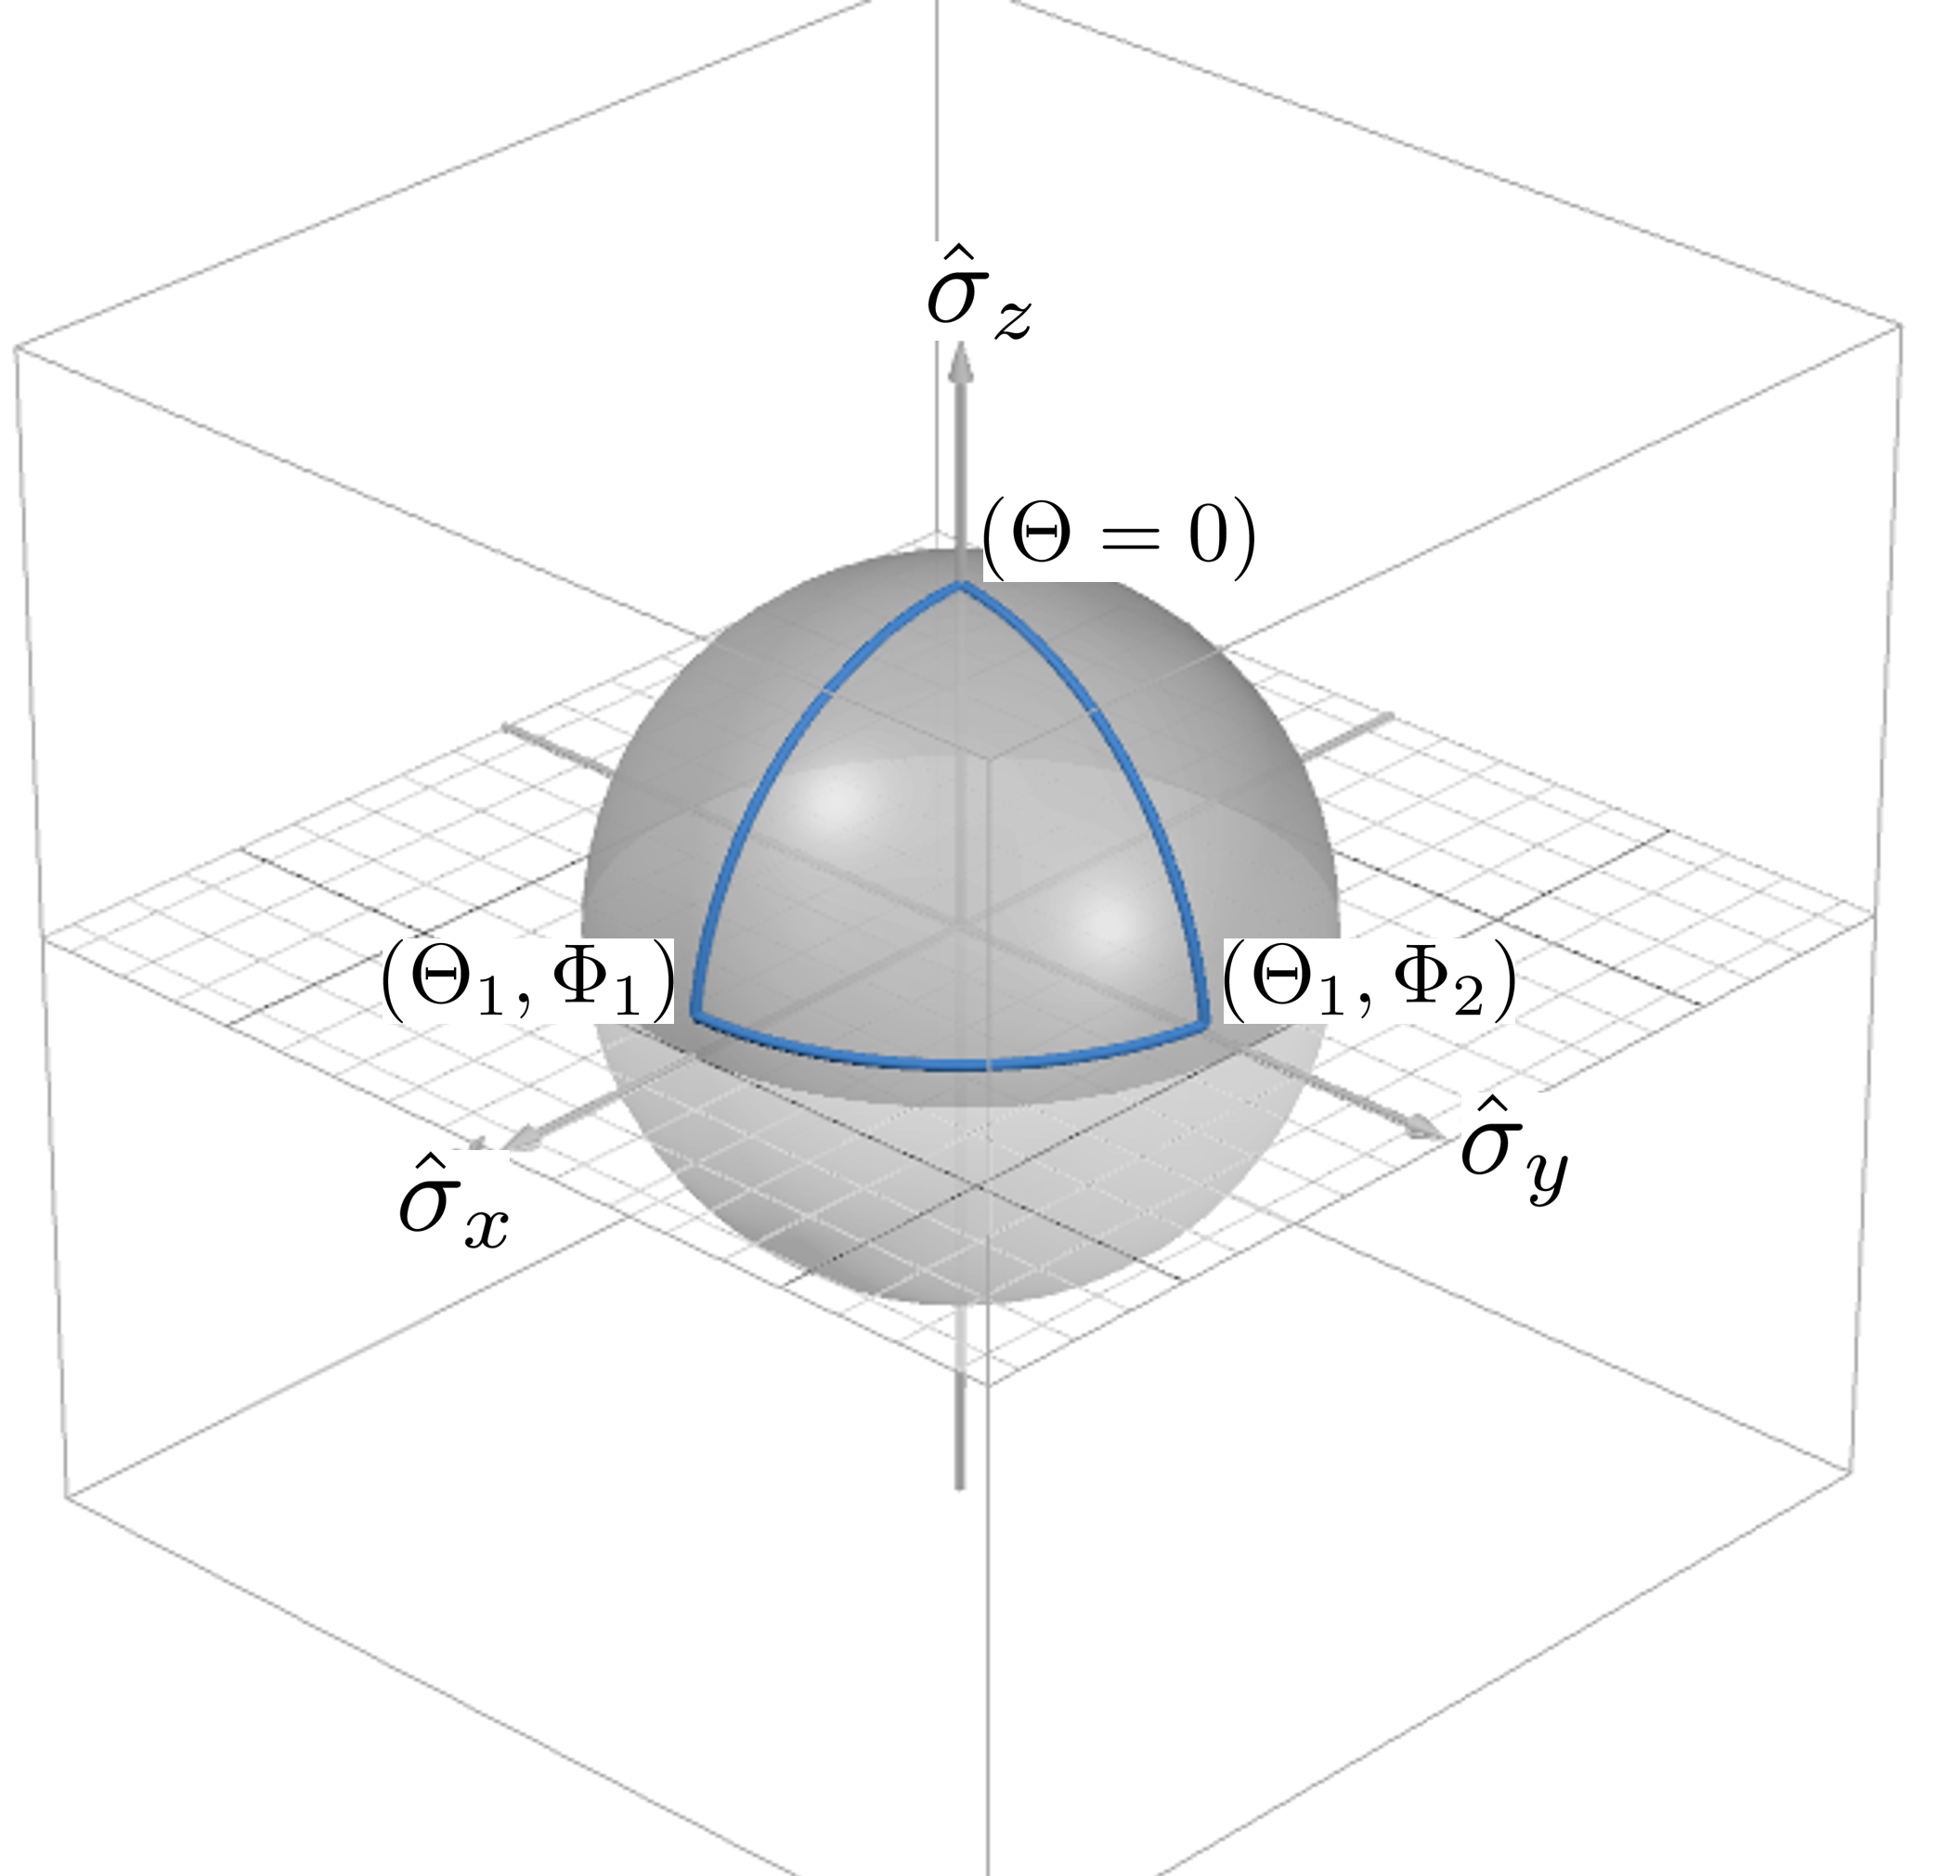
\includegraphics[scale=0.5]{figures/AAP_1.png}
  \caption{分極ベクトル$\bm{p}$の経路}
  \label{fig:AAP_1}
\end{figure}

\begin{figure}[htbp]
  \centering
  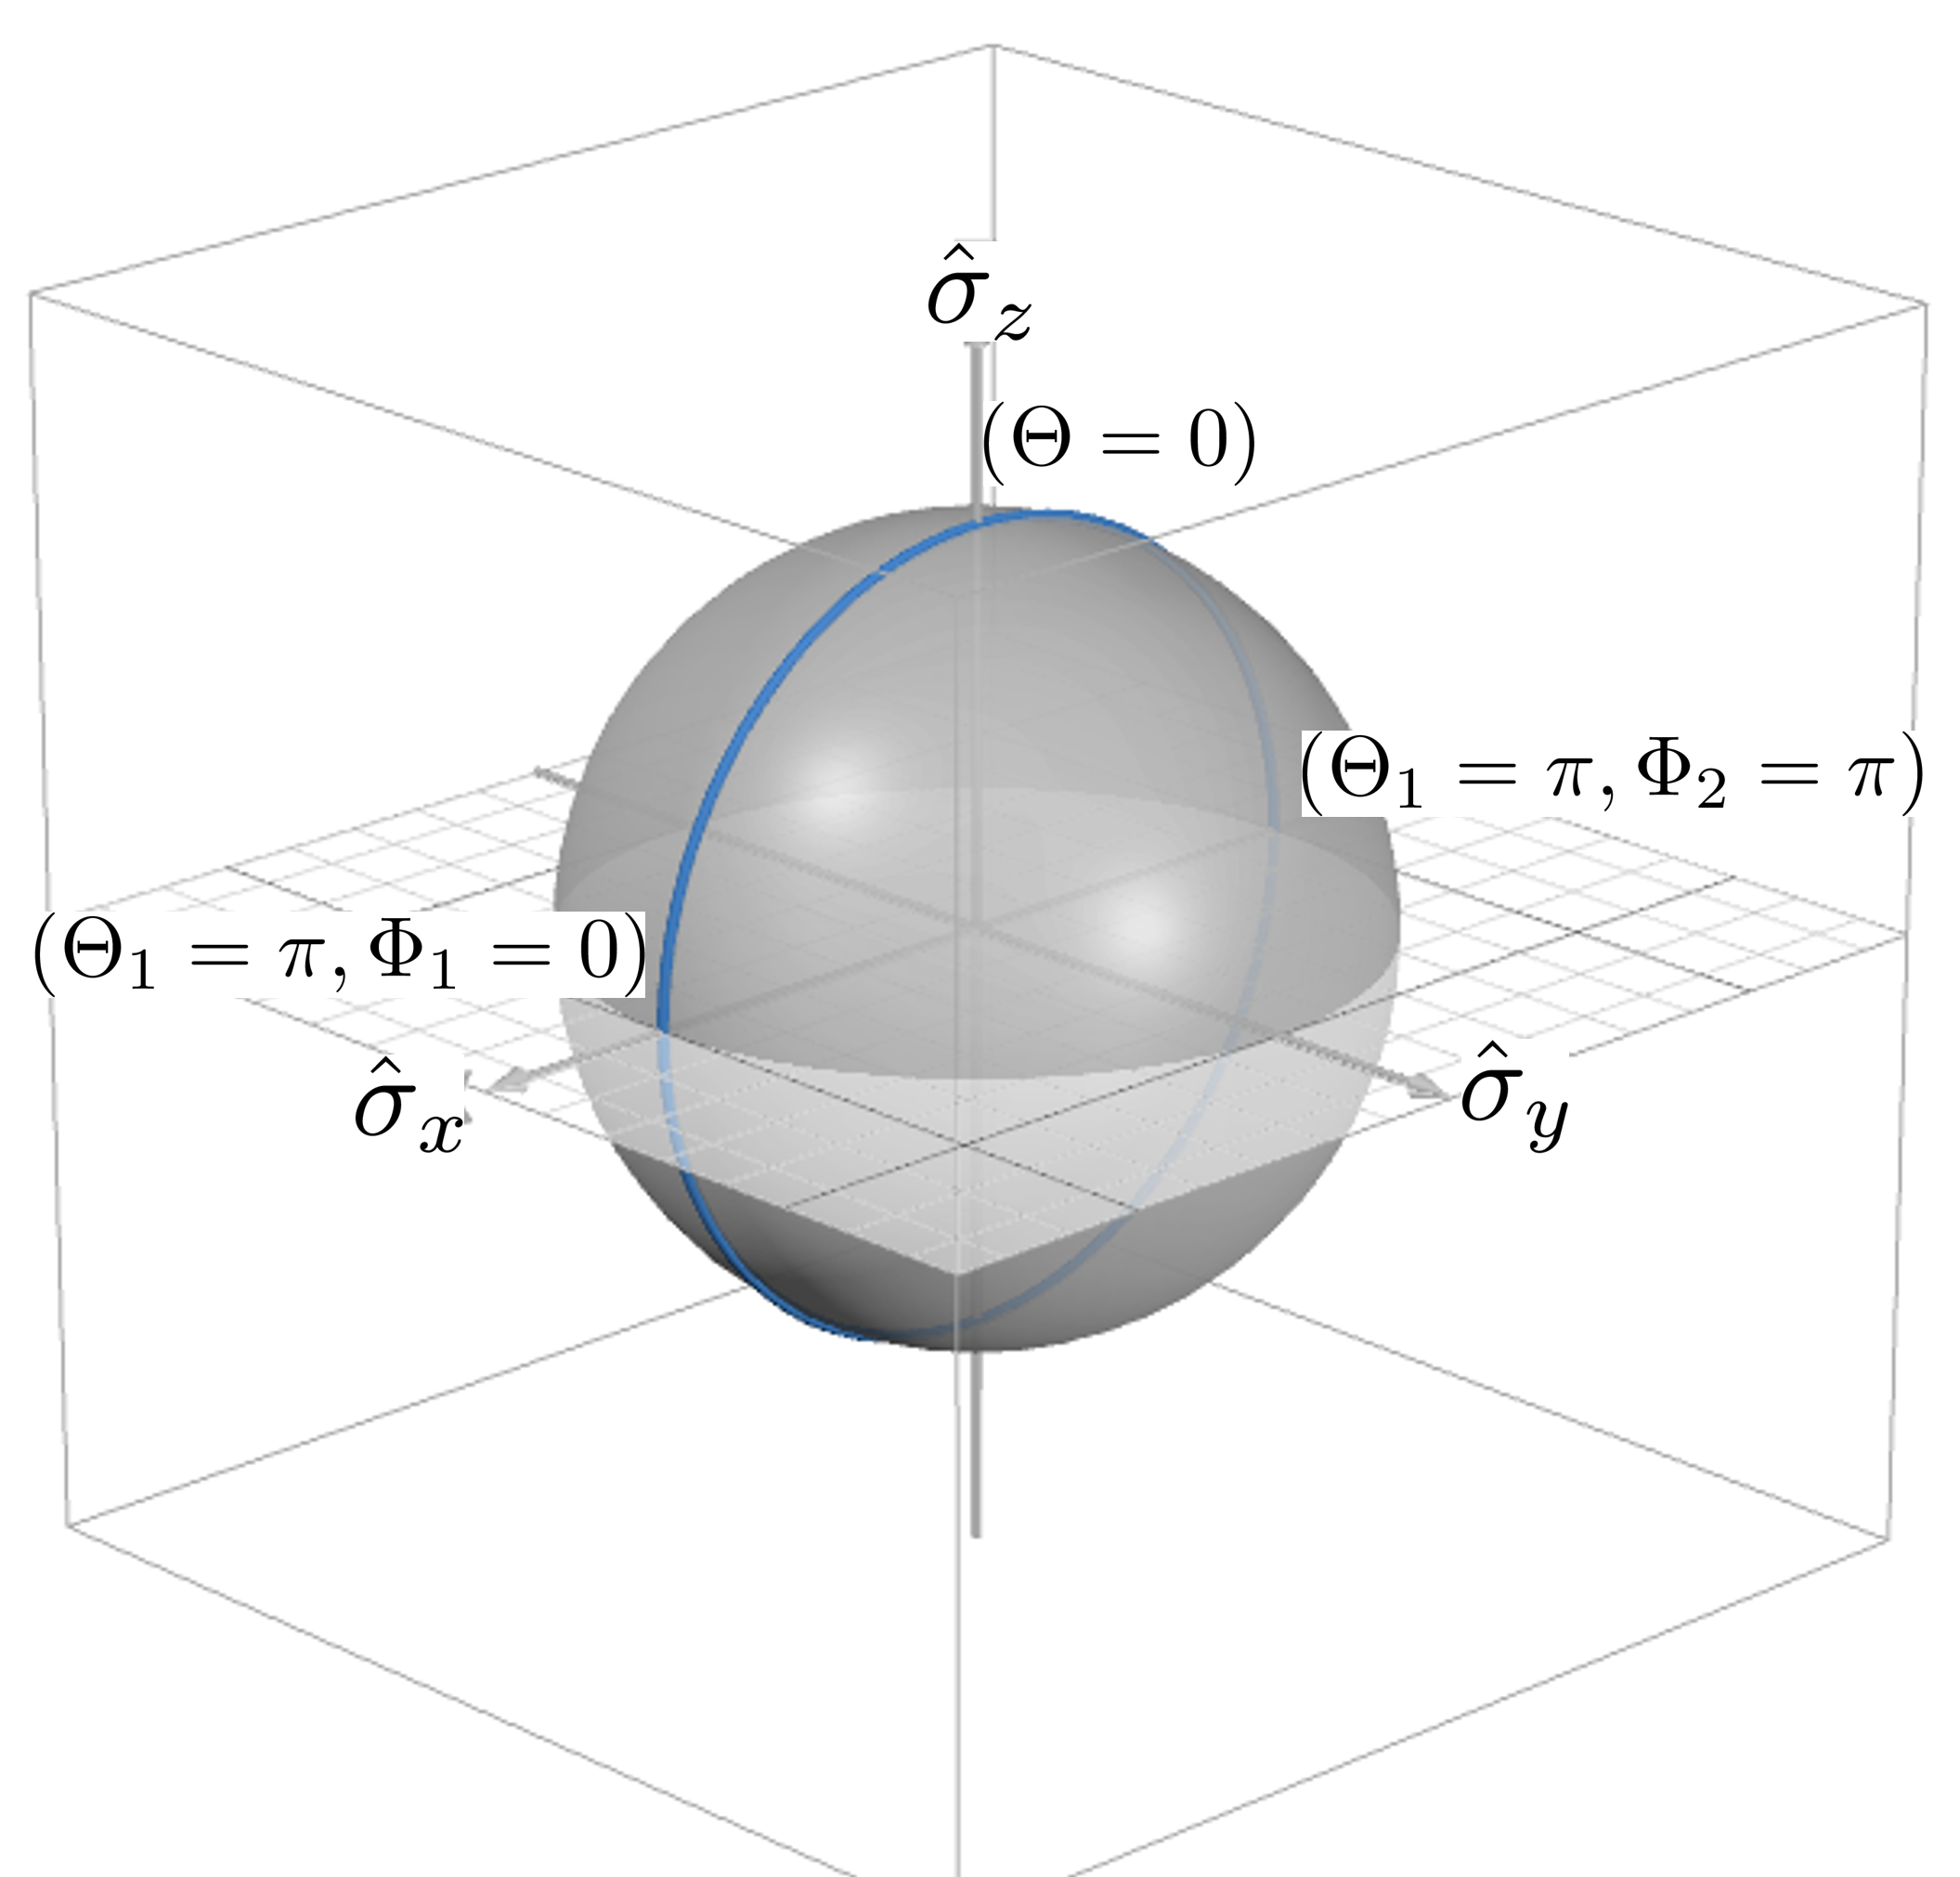
\includegraphics[scale=0.5]{figures/AAP_2.png}
  \caption{断熱極限における,分極ベクトル$\bm{p}$の経路}
  \label{fig:AAP_2}
\end{figure}


最後に,$2n$回目の準位交差で初期状態に戻る一般的な場合について,Aharonov-Anandan位相を求めておこう.式(\ref{cos_xi})で定義される$\xi$が,
\begin{equation}
  \xi = \frac{l}{2n} \pi \quad (l,n \text{は互いに素で,}0 < l < 2n) \label{xi_condition}
\end{equation}
のとき,$2n$回目の準位交差で,波動関数は符号を除いて初期状態に戻る.このことを確かめたければ,条件(\ref{xi_condition})を仮定して,式(\ref{psi_2m})を具体的に計算すればよい.


では,$2$回目の準位交差でAharonov-Ahandan位相を求めたときに用いた方法のように,まず動力学的位相から求めよう.系を4つの領域
\begin{enumerate}
\setcounter{enumi}{3}
\renewcommand{\labelenumi}{(\roman{enumi})}
  \item $t=0$から$t = \frac{\pi}{2\omega}$までの区間
  \item $t= \frac{\pi + 4k\pi}{2\omega}$から$t = \frac{3\pi + 4k\pi}{2\omega}$までの区間
  \item $t = \frac{3\pi + 4k\pi}{2\omega}$から$t = \frac{4\pi + 5k\pi}{2\omega}$までの区間 
  \item 最後のTLZ遷移から$t = \frac{2m\pi}{\omega}$までの区間
\end{enumerate}
に分割する.また,各領域における波動関数および動力学的位相をそれぞれ$\chi_d^{(\mathrm{x})}, \psi^{(\mathrm{x})} (\mathrm{x} = \mathrm{iv}, \mathrm{v}, \mathrm{vi}, \mathrm{vii})$とする.このとき,(iv)および(vii)の領域における動力学的位相は,$2$回目の準位交差でAharonov-Ahandan位相を求めたときと同様に,それぞれ$-\theta/2$である.また,(v)$t= \frac{\pi + 4k\pi}{2\omega}$から$t = \frac{3\pi + 4k\pi}{2\omega}$のときの動力学的位相$\chi_d^{(\mathrm{v})}$は,
\begin{align}
  -\left( 1 - 2q \left( \frac{\sin (2m-1) \xi}{\sin \xi} \right)^2 \right) \theta,
\end{align}
(vi)$t = \frac{3\pi + 4k\pi}{2\omega}$から$t = \frac{4\pi + 5k\pi}{2\omega}$のときの動力学的位相$\chi_d^{(\mathrm{vi})}$は,
\begin{align}
  -\left( 1 - 2q \left( \frac{\sin (2m) \xi}{\sin \xi}\right)^2\right) \theta,
\end{align}
であることが,$2$回目の準位交差でAharonov-Ahandan位相を求めたときと同様に計算できる.


したがって,
\begin{align}
  \chi_d
  &= - \theta - \sum_{m=1}^{2n-1} \left( 1 - 2q \left(\frac{\sin (2m) \xi}{\sin \xi}\right)^2\right) \theta\\
  &= -\theta - (2n-1) \theta + 2nq\frac{1}{\sin^2 \xi}\\
  &= -2n\theta (1-\frac{q}{\sin^2 \xi})
\end{align}
より,$2n$回目の準位交差で初期状態に戻る一般的な場合におけるAharonov-Anandan位相は,
\begin{equation}
  \chi_g = (n+l)\pi + 2n\theta \left( 1-\frac{q}{\sin^2 \xi} \right)
\end{equation}
である.$n=1$を代入すると,明らかに式(\ref{chi_g_AA})に一致する.